\subsection{Generación de señalamiento paso a paso}

	Al ejecutar el RNA, primero detectará todos los \textit{netElements}, sus coordenadas iniciales y finales en la topología, y el sentido en el que fueron definidas. El resultado obtenido se muestra en el Cóodigo \ref{lst:EJ1_1}.
	
	\begin{lstlisting}[language = {}, caption = Detección de \textit{netElements} por parte del RNA , label = {lst:EJ1_1}]
	###### Starting Railway Network Analyzer #####
	Reading .railML file
	Creating railML object
	Analysing railML object
	Analysing graph
	ne1 [810, 150] [1320, 150] >>
	ne2 [2970, 0] [2460, 0] <<
	ne8 [1320, 150] [1800, 150] >>
	ne9 [1320, 150] [1530, 360] >>
	ne12 [2460, 0] [1950, 0] <<
	ne13 [2460, 0] [810, -180] <<
	ne14 [1530, 360] [2970, 360] >>
	ne15 [1530, 360] [2970, 570] >>
	ne22 [1800, 150] [2970, 150] >>
	ne23 [1950, 0] [810, 0] <<
	ne24 [1800, 150] [1950, 0] >>
	The network is connected
	\end{lstlisting}
	
	Por ejemplo, el \textit{netElement} ne1 inicia en la coordenada (810;150) y finaliza en la coordenada (1320;150). El símbolo $>>$ indica que ne1 se encuentra definido de izquierda a derecha, ya que la componente x de la coordenada final es mayor a la de la coordenada inicial, teniendo la misma componente y. Además, se puede comprobar que la lista obtenida en consistente con la Figura \ref{fig:EJ1_2}. Por ejemplo, ne1, ne8 y ne9 comparten la coordenada (1320;150), que coincide con la coordenada del cambio de vías Sw04.
	
	A continuación, el RNA detectará la infraestructura ferroviaria, las curvas peligrosas y los puntos medios de los netElements que el RNA considera demasiado largos. El resultado de este proceso se puede visualizar en el Código \ref{lst:EJ1_2} y puede leerse también en el archivo Infrastructure.RNA.
	
	\begin{lstlisting}[language = {}, caption = Detección de puntos críticos por parte del RNA , label = {lst:EJ1_2}]
	Analysing infrastructure --> Infrastructure.RNA
	Detecting Danger --> Safe_points.RNA
	ne1 has a Middle point @ [1065.0, 150]
	ne2 has a Middle point @ [2715.0, 0]
	ne8 has a Middle point @ [1560.0, 150]
	ne12 has a Middle point @ [2205.0, 0]
	ne13 has a Platform[plf75] @ [1564, 180]
	ne13 has a LevelCrossing[lcr74] @ [1362, 180]
	ne13 has a Curve(2 lines) @ [[2280, -180]]
	ne14 has a Platform[plf68] @ [2490, -360]
	ne14 has a LevelCrossing[lcr69] @ [1945, -360]
	ne15 has a Curve(2 lines) @ [[1740, 570]]
	ne22 has a RailJoint[J15] @ [2452, 150]
	ne23 has a RailJoint[J14] @ [1284, 0]
	\end{lstlisting}
	
	Una vez que el RNA detectó cada punto crítico de la red ferroviaria, procede a generar el señalamiento. El orden de generación no es importante, pero para poder describirlo de forma consistente se iniciará generando el señalamiento para proteger los finales de vías, las junturas entre rieles, las plataformas, los cruces de vía y los cambios de vías. Luego se procederá a mostrar el señalamiento pre y post simplificación. Las señales generadas para proteger los finales de vías relativos y absolutos son ilustradas en la Figura \ref{fig:EJ1_3}.
	
	\begin{figure}[H]
		\centering
		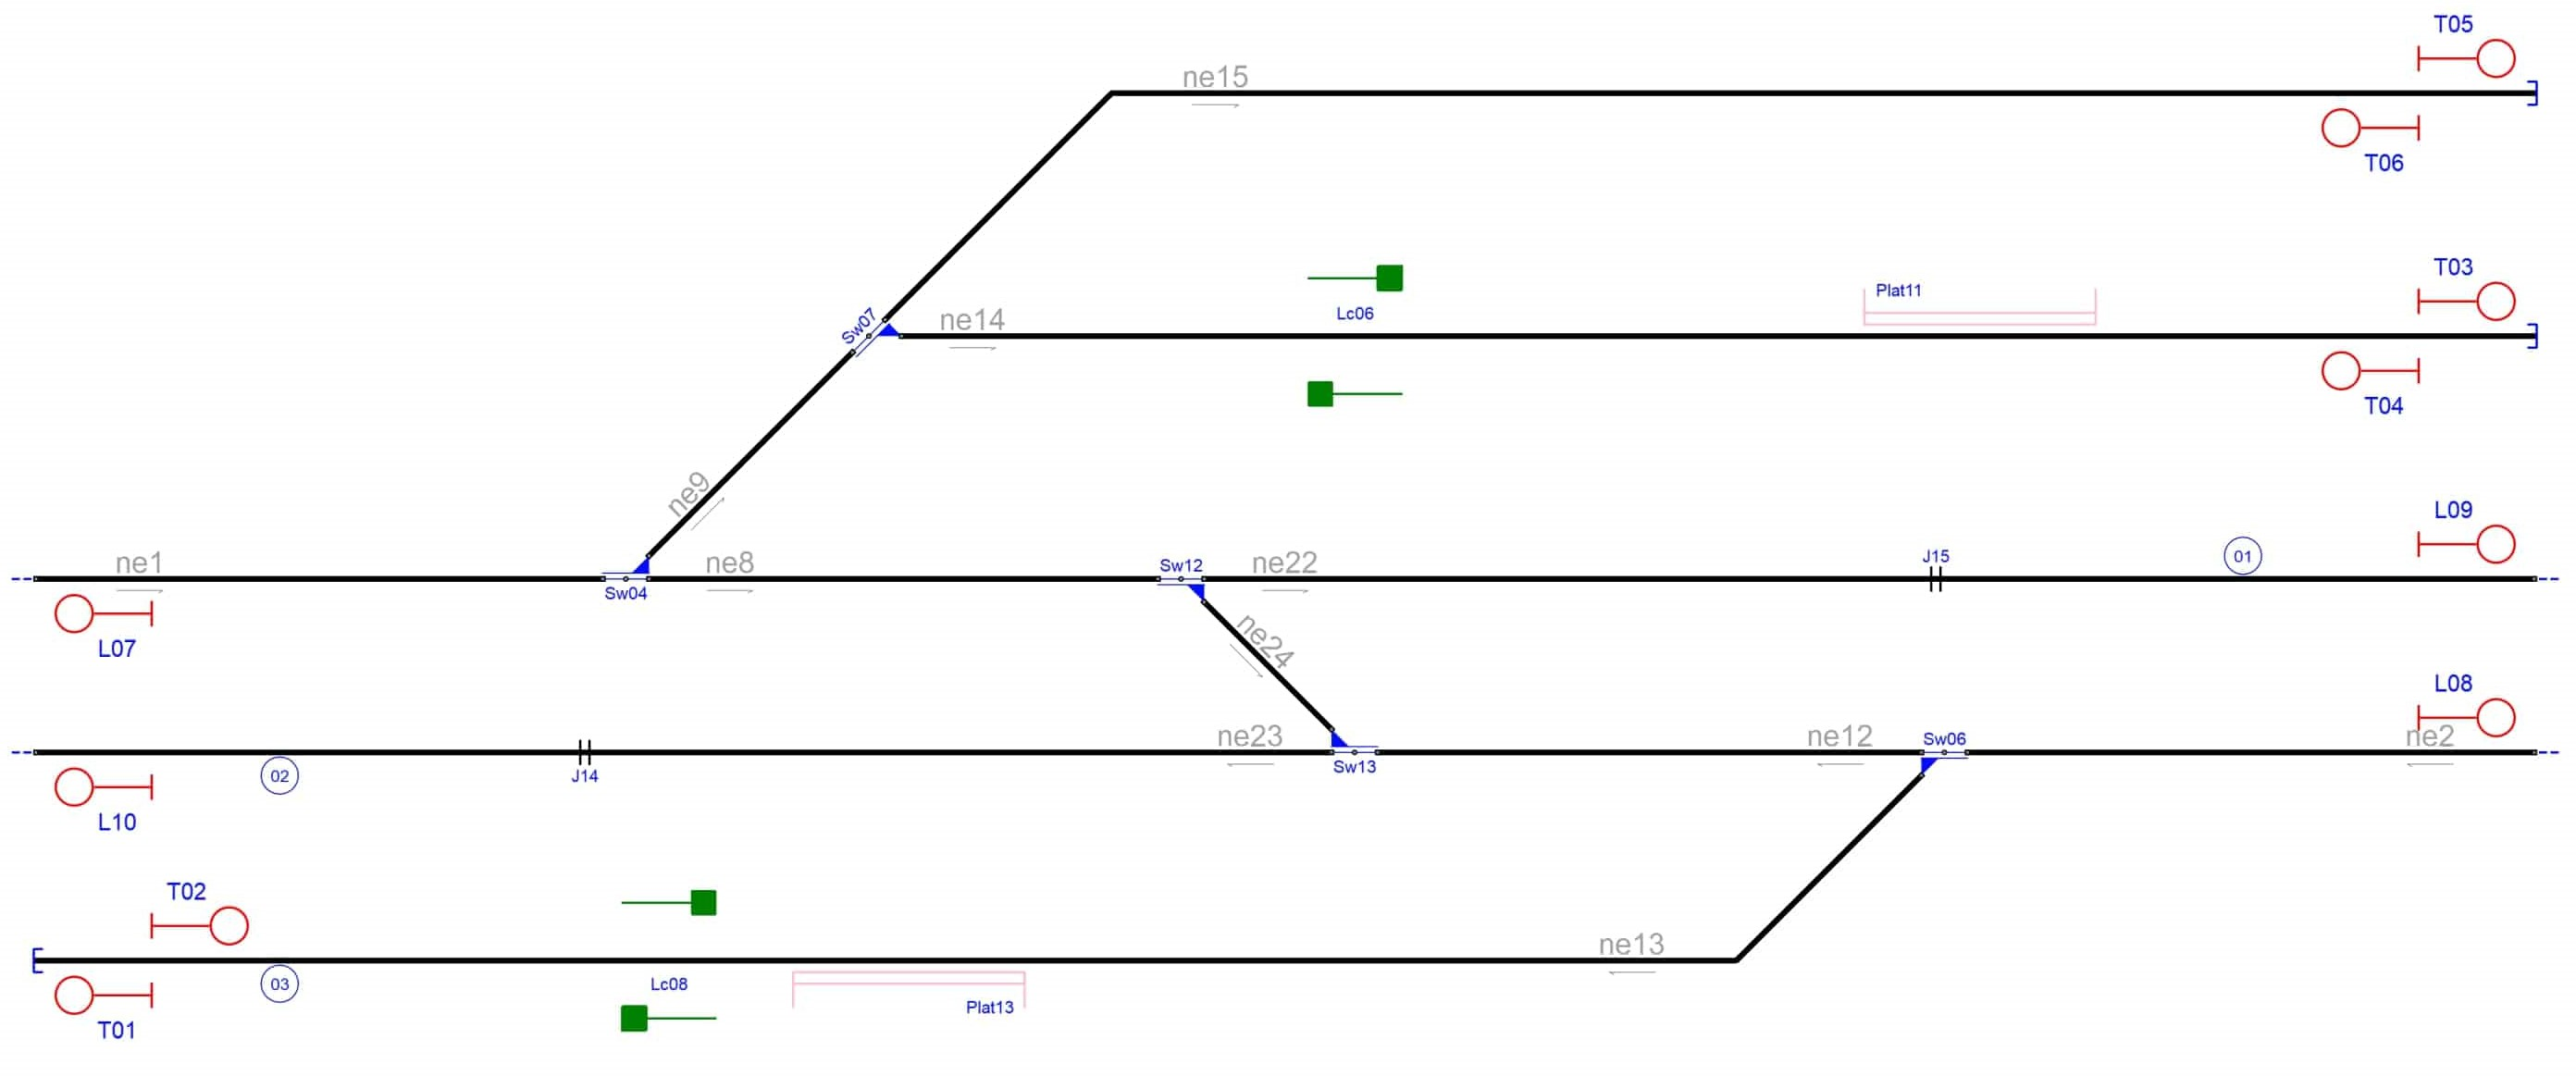
\includegraphics[width=1\textwidth]{resultados-obtenidos/ejemplo1/images/1_step1.png}
		\centering\caption{Señalamiento generado por el RNA para proteger el fin de vía.}
		\label{fig:EJ1_3}
	\end{figure}
	
	Los finales de vías absolutos son protegidos por las señales de parada T01, T03, T05 y las señales de partida son T02, T04 y T06. A su vez, los finales de vías relativos poseen las señales de parada L07, L08, L09 y L10, cercanos al límite del externo del \textit{netElement} al que pertenecen.
	
	La Figura \ref{fig:EJ1_4} ilustra la generación de señales destinadas a proteger las junturas entre los rieles. Las señales generadas son J11, J12, J13 y J14, indicadas en color rojo. De no existir junturas que proteger, el RNA salteará este paso.
	
	\begin{figure}[H]
		\centering
		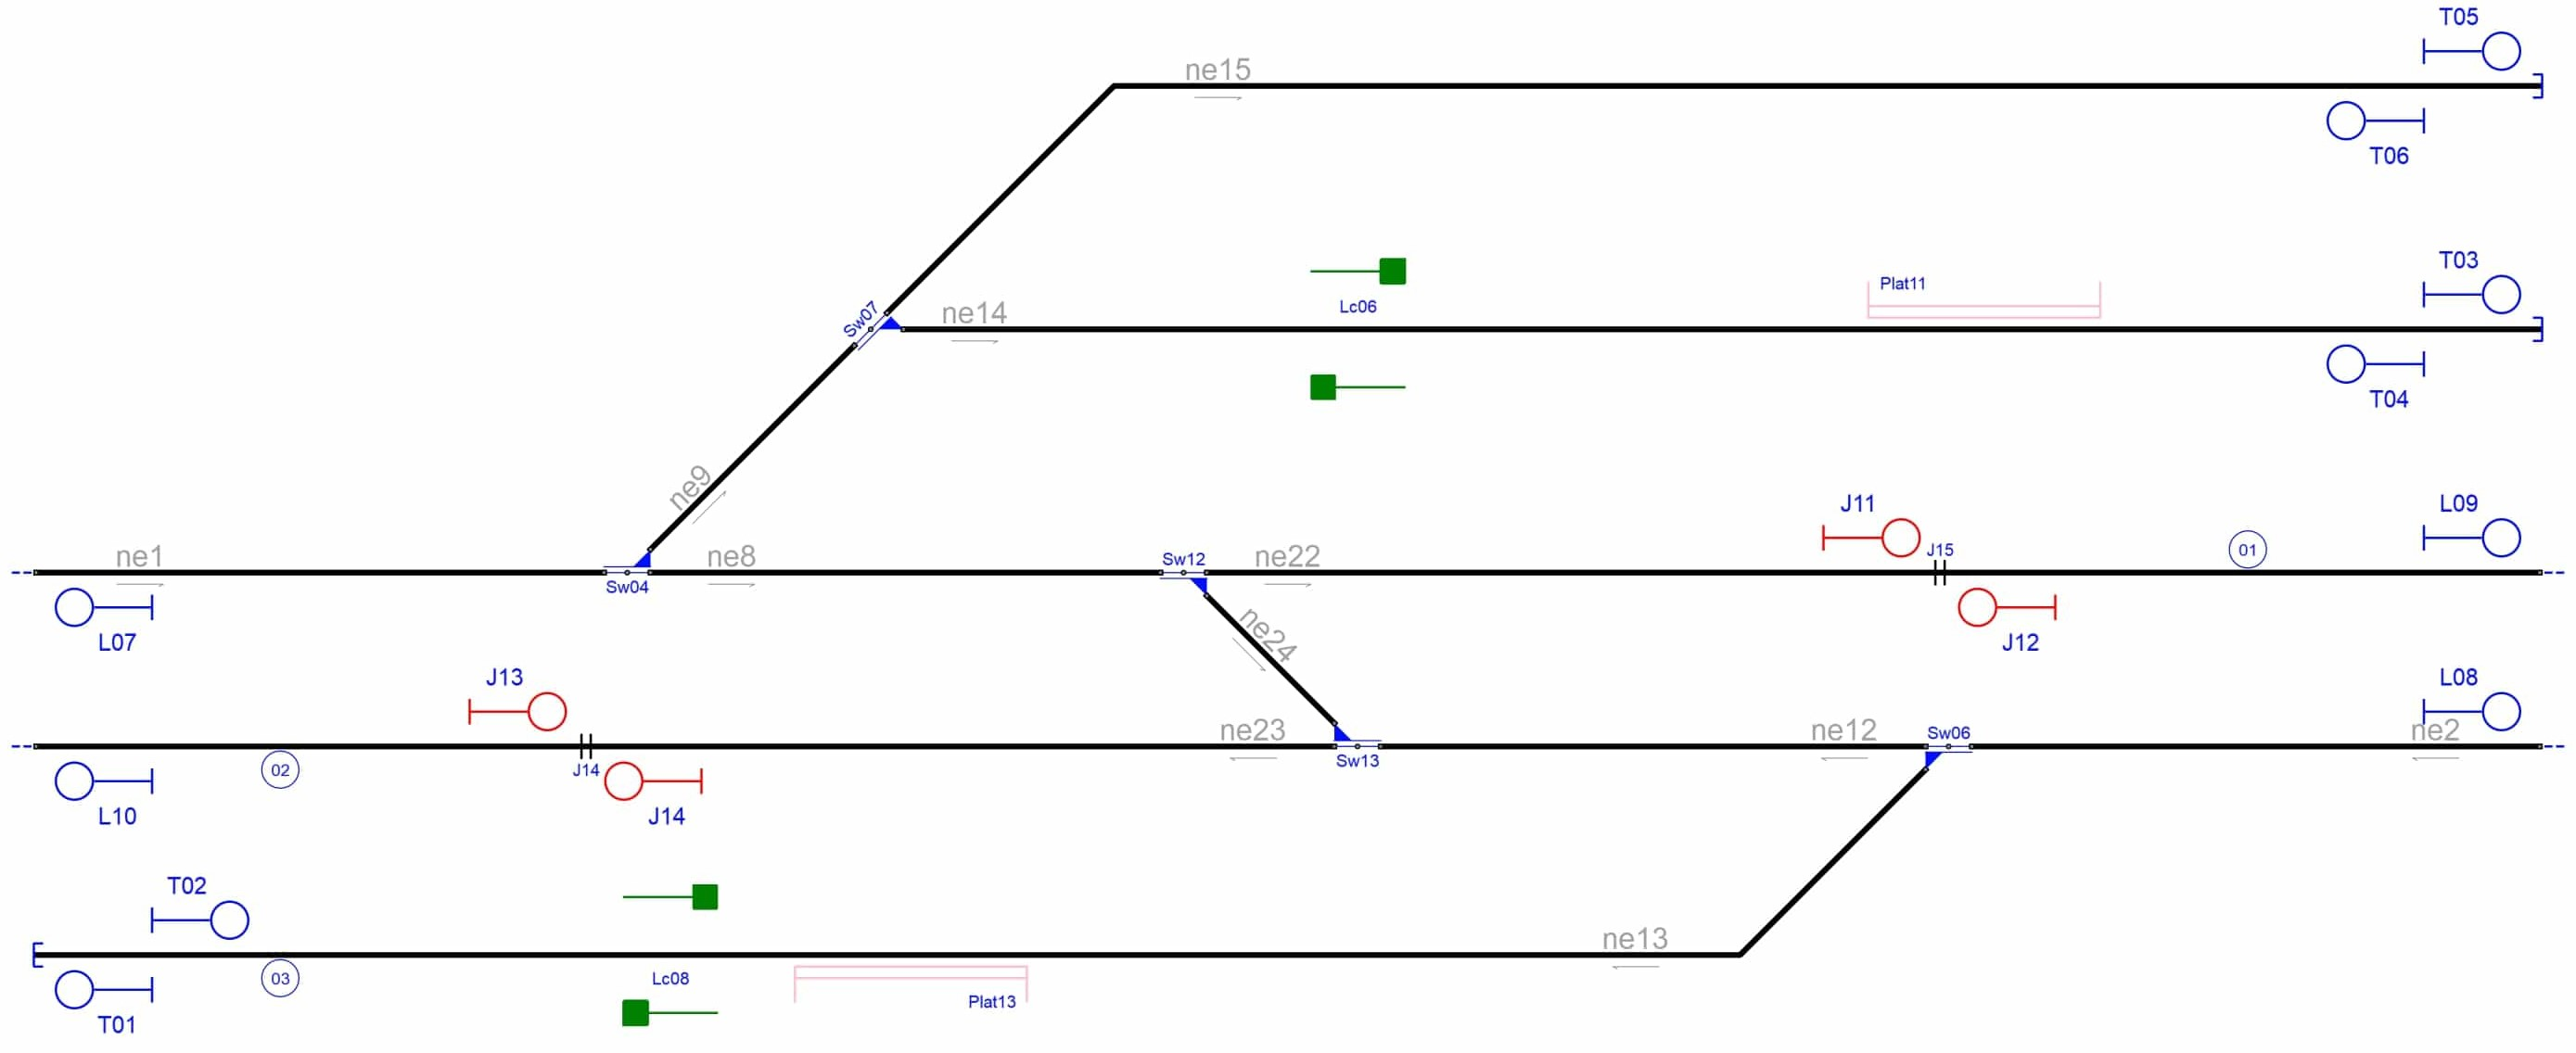
\includegraphics[width=1\textwidth]{resultados-obtenidos/ejemplo1/images/1_step2.png}
		\centering\caption{Señalamiento generado por el RNA para proteger las junturas.}
		\label{fig:EJ1_4}
	\end{figure}
	
	Al generar el señalamiento para proteger la infraestructura, tal como se explicó en la Sección \ref{sec:horizontal}, el Algoritmo \ref{alg:horizontal} simplificará las señales entre dos elementos ferroviarios si no existe espacio suficiente entre ellos, tal como sucede con los elementos levelCrossing8 y Platform13. El señalamiento generado para proteger las plataformas y los cruces de vía se ilustra en rojo en la Figura \ref{fig:EJ1_5}. Las señales generadas para proteger las plataformas son las señales de partida P18, P19 y P20, mientras que las señales que protegen los cruces de vía son las señales X15, X16 y X17.
		
	\begin{figure}[H]
		\centering
		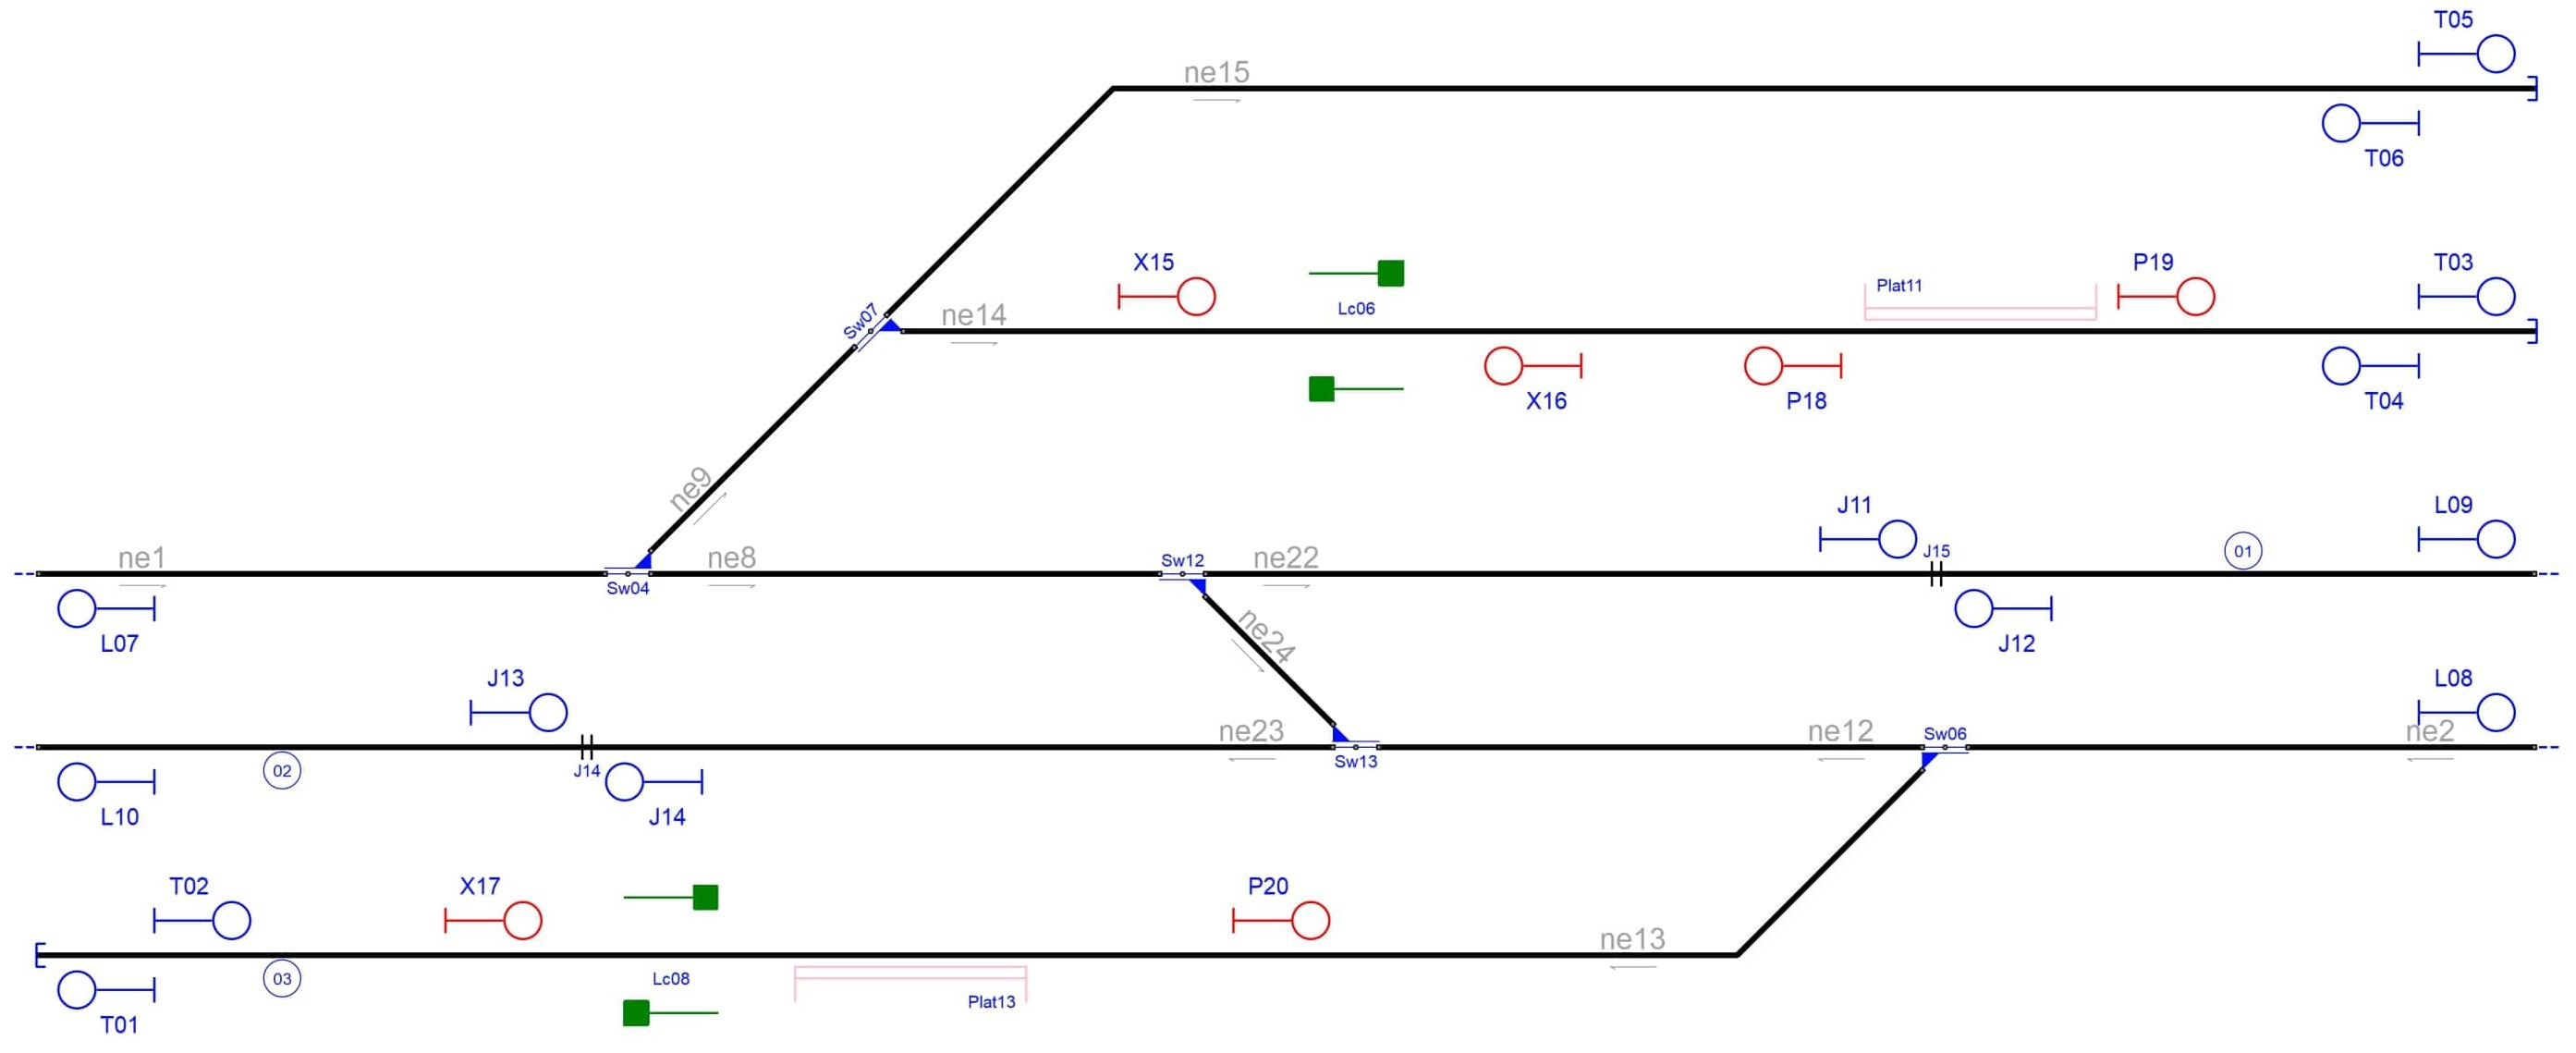
\includegraphics[width=1\textwidth]{resultados-obtenidos/ejemplo1/images/1_step3.png}
		\centering\caption{Señalamiento generado por el RNA para proteger plataformas y cruces de vía.}
		\label{fig:EJ1_5}
	\end{figure}
	
	El RNA generó las señales S22, C21, H23 y H24 para proteger el cambio de vías Sw04; las señales S27, C25, B26 y H28 para proteger el cambio de vías Sw06; las señales C29 y B30 para proteger el cambio de vías Sw07; las señales S32, C31 y H33 para proteger el cambio de vías Sw12 y las señales S35, C34 y H36 para proteger el cambio de vías Sw13. Las señales mencionadas se encuentran resaltadas en rojo en la Figura \ref{fig:EJ1_6}.
	
	\begin{figure}[H]
		\centering
		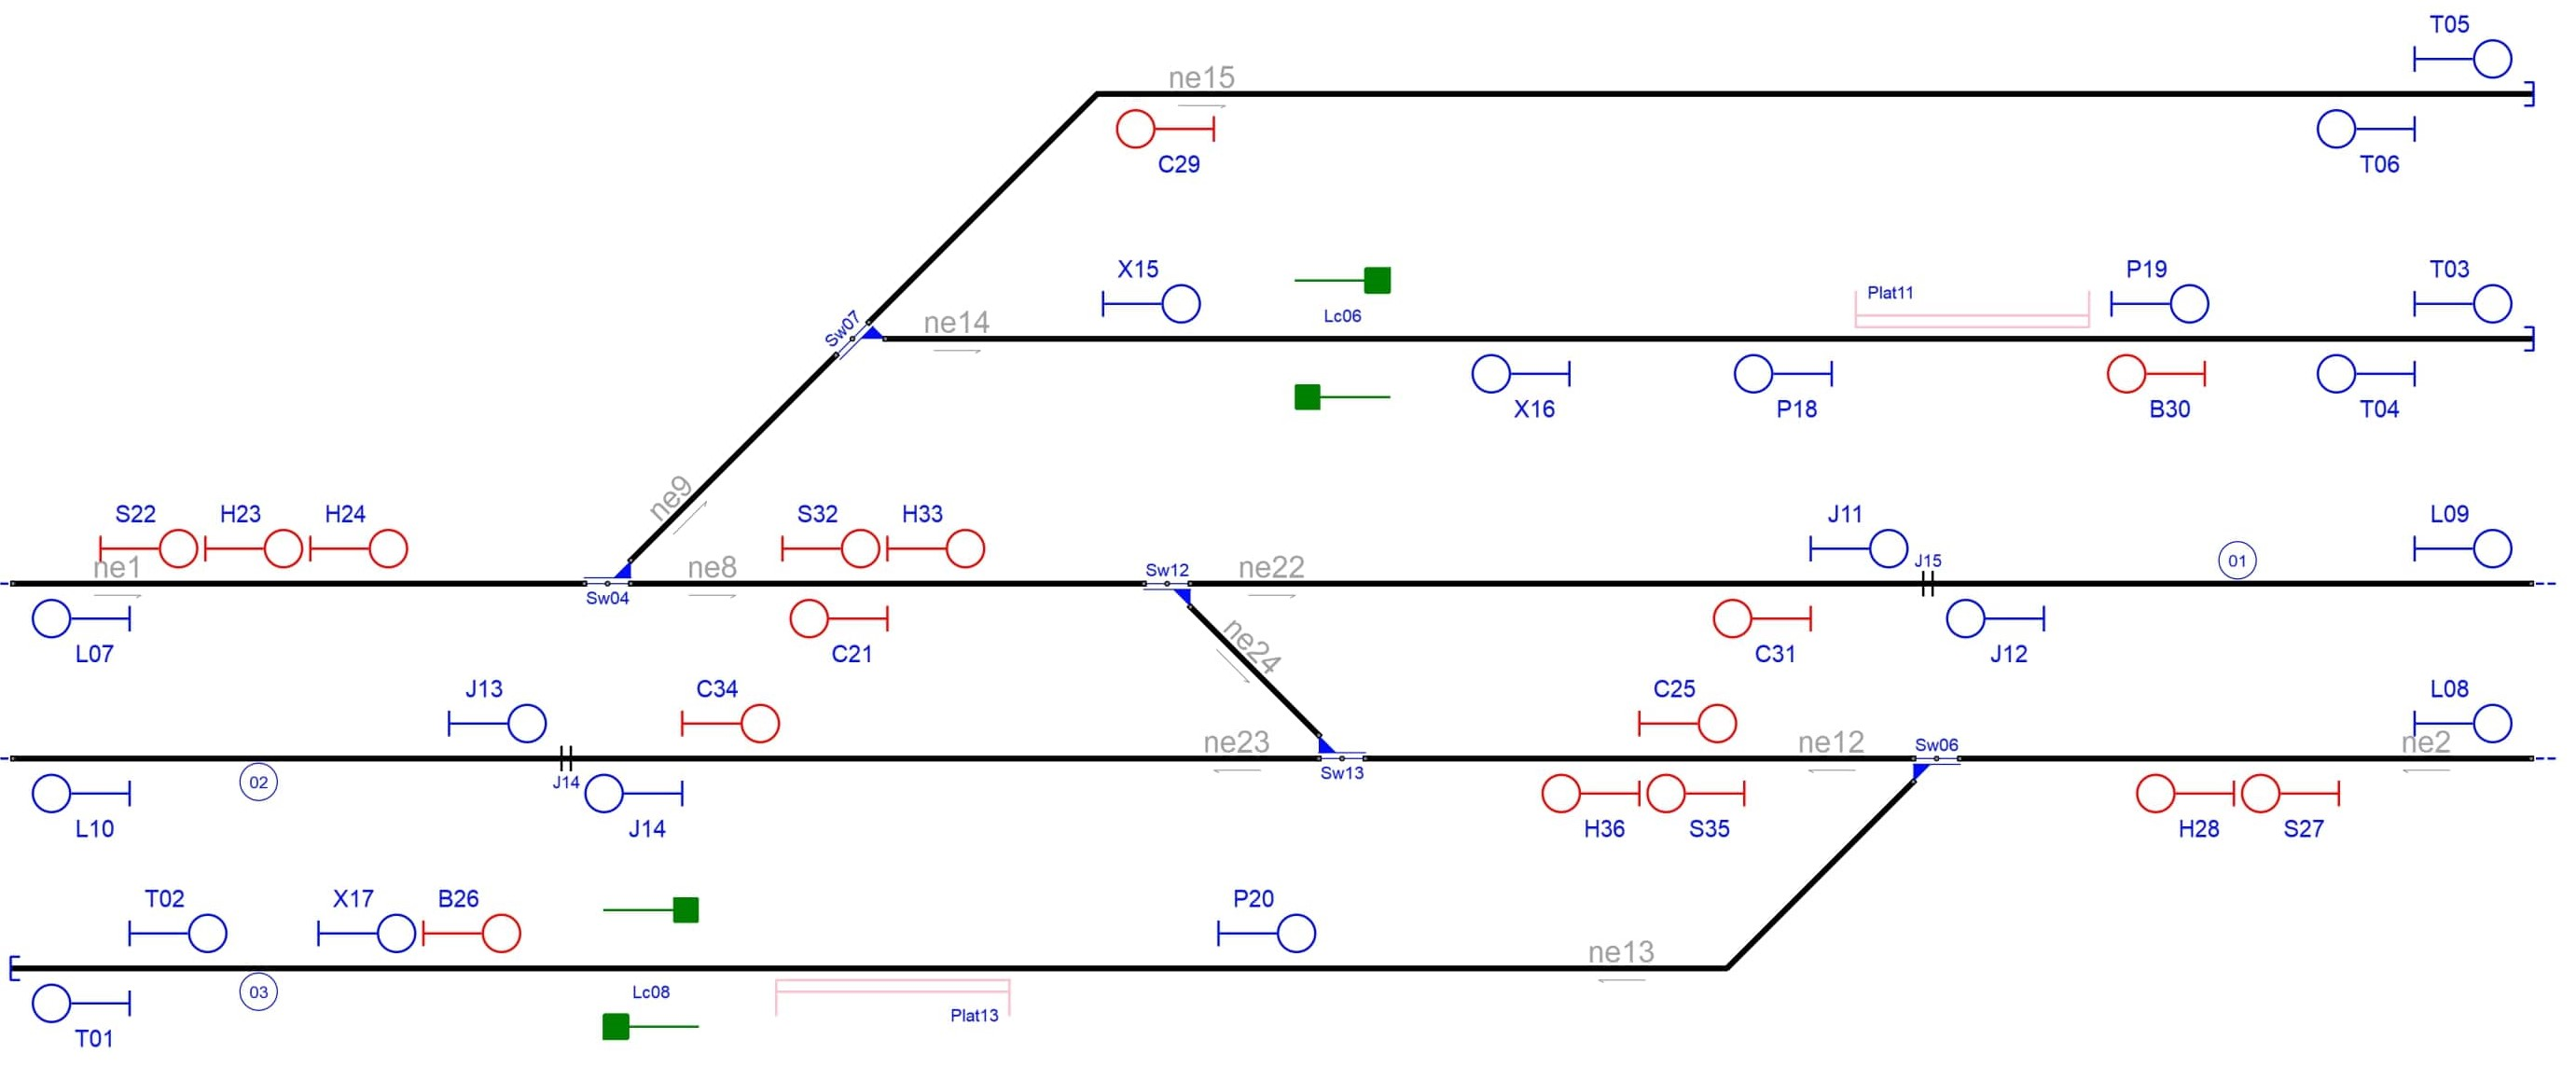
\includegraphics[width=1\textwidth]{resultados-obtenidos/ejemplo1/images/1_step4.png}
		\centering\caption{Señalamiento generado por el RNA para proteger los cambios de vías.}
		\label{fig:EJ1_6}
	\end{figure}
	
	Una vez obtenido todo el señalamiento, el RNA procede a simplificar las señales redundantes, repetidas o cuyas funciones o ubicaciones se superponen entre sí. El proceso de simplificación de señales fue explicado en la Sección \ref{sec:simplificacion}. El Algoritmo \ref{alg:vertical} de herencia vertical fue aplicado en las señales B entre los cambios de vías Sw12 y Sw13, desplazando las señales hasta convertirlas en las señales H33 y H36 respectivamente. Análogamente, las señales C y S del \textit{netElement} se convirtieron en las señales H23 y H24 respectivamente.
	
	Las señales simplificadas al aplicar el Algoritmo \ref{alg:horizontal} de herencia horizontal son: X17, P18, P19, B26, B30, C31 y C34. Las señales X17 y B26 fueron eliminadas por su cercanía con la señal T02, con la cual comparten dirección y sentido. Lo mismo ocurre entre el par de señales P18/B30 y la señal T04; entre las señales P19 y T03; entre las señales C31 y J12; y entre las señales C34 y J13. En todos los casos, se aplicó el Algoritmo \ref{alg:horizontal}, diseñado para agrupar objetos cercanos como un único objeto, y así generar el señalamiento acorde a los elementos contenidos en cada extremo del nuevo elemento contenedor.
	
	Finalmente, las señales son simplificadas aplicando el Algoritmo \ref{alg:reduction} de eliminación por prioridad de señales. El resultado de este proceso es detallado en el Código \ref{lst:EJ1_3}.
	
	\begin{lstlisting}[language = {}, caption = Reducción de señalamiento por prioridad de señales, label = {lst:EJ1_3}]
	Reducing redundant signals
	removing sig17 for sig02
	removing sig26 for sig02
	removing sig19 for sig03
	removing sig30 for sig04
	removing sig31 for sig12
	removing sig34 for sig13
	removing sig18 for sig30
	\end{lstlisting}
	
	El resultado de la simplificación del señalamiento se ilustra en la Figura \ref{fig:EJ1_7}.
	
	\begin{figure}[H]
		\centering
		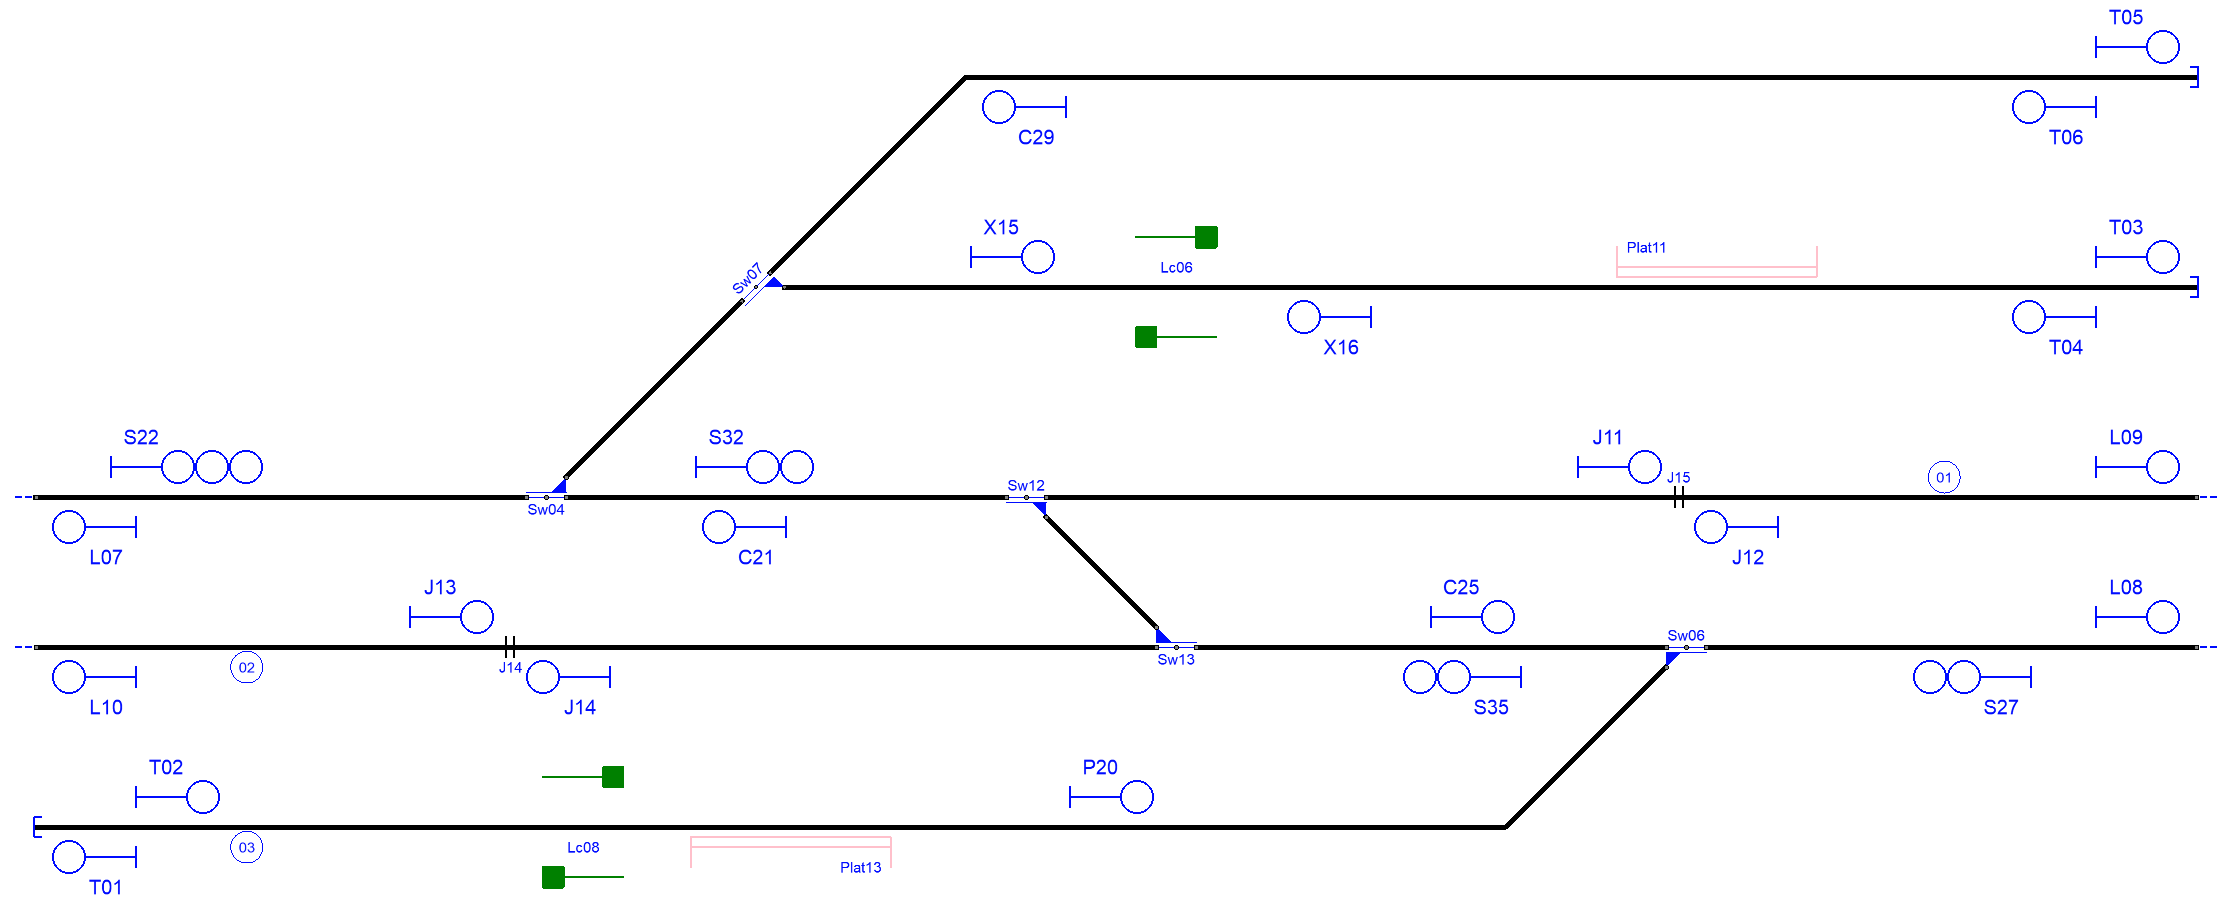
\includegraphics[width=1\textwidth]{resultados-obtenidos/ejemplo1/images/1_RNA.png}
		\centering\caption{Señalamiento generado y simplificado por el RNA.}
		\label{fig:EJ1_7}
	\end{figure}
	
	Al finalizar la generación del señalamiento, el RNA debe detectar todas las posibles rutas admitidas por la red para crear la tabla de enclavamientos. El RNA exporta los resultados del análisis en los siguientes cuatro documentos: Infrastructure.RNA (Apéndice \ref{sec:infrastructureRNA}), SafePoint.RNA (Apéndice \ref{sec:safePointsRNA}), Signalling.RNA (Apéndice \ref{sec:signallingRNA}) y Routes.RNA (Apéndice \ref{sec:routesRNA}).